
%% Scientific data, equations, and citation mapping retained.

\documentclass[pdflatex,sn-apa]{sn-jnl}

\usepackage[T1]{fontenc}
\usepackage{amsmath}
\usepackage{amssymb}
\usepackage{booktabs}
\usepackage{tabularx}
\usepackage{tikz}
\usepackage{upgreek}
\usepackage{lineno}
\usetikzlibrary{arrows.meta}
\usepackage{url}

\setcounter{secnumdepth}{0}

\begin{document}


\title{Distinguishing microplastic and oil pollutants at the water surface using multi-angle LWIR polarization imaging}


\author*[1]{\fnm{Luk\'a\v{s}} \sur{Krauz}}\email{krauzluk@fel.cvut.cz}
\author[1]{\fnm{Artem} \sur{Efremov}}
\author[1]{\fnm{Milo\v{s}} \sur{Kl\'ima}}
\author[1]{\fnm{Jan} \sur{Bedn\'a\v{r}}}
\author[1]{\fnm{Petr} \sur{P\'ata}}

\affil[1]{\orgdiv{Department of Radioelectronics, Faculty of Electrical Engineering},
\orgname{Czech Technical University in Prague},
\orgaddress{\street{Technick\'a 2}, \city{Prague 6}, \postcode{166 27}, \country{Czech Republic}}}

\abstract{
Pollution of the water surface by microplastics and oils is a significant problem and requires complementary imaging methods for their fast identification. Among these new methods, polarization imaging can be considered a promising modality. Therefore, this paper assesses the use of multi-angle long-wave infrared (LWIR) polarization imaging for distinguishing selected microplastics, oils, and the water surface under active illumination. Nine plastic materials and five oils were measured at five illumination and observation geometries using a rotating linear analyzer. The degree of linear polarization (DoLP) and angle of linear polarization (AoLP) were evaluated for the individual samples. The main difference was observed in DoLP. The root-mean-square (RMS) DoLP of the microplastic group remained within the range $5.12\times10^{-4}$--$6.77\times10^{-4}$, while the RMS DoLP of the oil group increased from $1.85\times10^{-2}$ to $1.18\times10^{-1}$ toward larger illumination and observation angles. In terms of DoLP, the water-surface reference remained between the two pollutant groups for all five geometries. Control active illumination measurements also showed substantially higher DoLP for water and vegetable oil with active illumination than with the source blocked, while polypropylene remained within the same very low DoLP range for both illumination conditions. The AoLP characteristics showed substantially greater overlap between the pollutant groups. Under the investigated laboratory conditions, DoLP therefore provided a clear distinction among the investigated microplastics, the water-surface reference, and the oil layers, while AoLP provided weaker separation.

}



% \keywords{microplastics, oils, water pollution, LWIR, DoLP, polarization imaging}
\keywords{environmental monitoring, surface contamination,
DoLP, AoLP, thermal imaging, active illumination}




\linenumbers
\maketitle

% \section*{Highlights}
% \begin{itemize}
% \item DoLP distinguished selected microplastics, water, and oil layers.
% \item Investigated microplastics remained below the water-reference DoLP.
% \item All investigated oils remained above the water-reference DoLP.
% \item Active LWIR illumination increased DoLP for water and vegetable oil.
% \item AoLP overlapped between the microplastic and oil groups.
% \end{itemize}

% ------------------------------------------------------------------
\section{Introduction}
% ------------------------------------------------------------------

Water-surface pollution by plastic waste and oils represents a severe environmental problem due to their widespread occurrence and potential harmful effects on aquatic ecosystems~\citep{Beyer2016,Yusuf2022}. A global modelling study estimated annual riverine inputs of plastic waste to the ocean at 1.15--2.41 million tonnes~\citep{Lebreton2017}. Accidental oil spills also remain an important source of marine pollution. For example, in 2024, approximately 10,000 tonnes of oil were reported to have been released in tanker incidents~\citep{ITOPF2025}.

In recent years, increasing attention has been paid to microplastics, which are commonly defined as plastic particles smaller than 5~mm~\citep{Hartmann2019,Nihei2024}. Their small dimensions and heterogeneous morphology and composition make the reliable identification of microplastics at the water surface severely challenging. Due to their problematic detectability, most approaches rely on laboratory analyses such as microscopic and spectroscopic techniques, or their combination~\citep{HidalgoRuz2012,Prata2019,Yusuf2022}. Nevertheless, complementary imaging methods are increasingly investigated~\citep{Fang2023,Zhu2024}. For the spectral analysis, various spectral regions are used. Promisingly, in recent years, near infrared-based and shortwave-infrared-based hyperspectral imaging has demonstrated the identification of several polymer types in water-related samples as well as the automated classification of smaller and irregular plastic particles~\citep{Schmidt2018,Shan2019,Gebejes2024,Holt2025,Chatzitoulousis2026}.

Beyond laboratory conditions, remote sensing of floating plastic pollution has also exploited imaging in various spectral bands from the visible to the shortwave-infrared region to detect larger debris or accumulated litter~\citep{GoddijnMurphy2018,MartinezVicente2019,Cozar2024}. In addition, thermal infrared or long-wave infrared (LWIR) sensing may provide a complementary mechanism for plastic analysis. For example, a radiative-transfer study~\citep{GoddijnMurphy2019} showed that the thermal infrared response to floating plastic depends strongly on the temperature difference between the water surface and its surroundings and on the fraction of the surface covered by plastic. Previous laboratory LWIR measurements have also demonstrated diagnostic reflectance features of naturally dried plastic litter~\citep{Garaba2020}. Additionally, UAV experiments confirmed measurable thermal contrast for larger floating plastic targets under field conditions~\citep{GoddijnMurphy2022}. However, strong absorption of thermal radiation by water limits direct observation mainly to materials located at or near the surface~\citep{GoddijnMurphy2022,GoddijnMurphy2024}. Thus, reliable and direct LWIR remote assessment of individual microplastic-sized particles remains particularly challenging. 

In addition to the standard intensity image captured from a polluted scene, it is also possible to exploit other imaging modalities or characteristics of electromagnetic radiation, such as polarization. Polarization imaging or polarimetry can provide additional information related to material properties~\citep{Tominaga2008}, surface structure~\citep{Stolz2012}, roughness~\citep{Terrier2008}, and observation geometry~\citep{Tyo2006}. For example, previous studies on water surfaces showed that LWIR thermal radiation is slightly linearly polarized and that the polarization response changes strongly with viewing geometry~\citep{Shaw1999,Shaw2001}. Moreover, LWIR polarization signatures may also depend on the radiative state of the target and its optical background, since under specific conditions, thermal equilibrium can suppress the observed polarization signature~\citep{Tyo2007}. Therefore, measurement geometry and illumination conditions are important parameters in the interpretation of LWIR polarimetric data.

In the past years, LWIR polarimetry has already shown considerable potential for the analysis of oil layers on water. \citet{Zhang2014} created a prediction model within the 8--14~$\upmu$m range, showing stronger polarization contrast compared to radiation contrast for crude oil at the water surface under many viewing conditions. Subsequently, experimental studies demonstrated enhanced oil--water contrast and discrimination of selected oil products using infrared polarization information~\citep{Chenault2018,Fu2022,Sun2023}. Polarization has also been investigated for microplastics, but under significantly different measurement configurations. These polarization assessment approaches include polarized light scattering in water~\citep{Liu2021,Liu2024}, polarization-sensitive holographic imaging~\citep{Valentino2022}, and Mueller-matrix measurements of suspended or separately measured particles~\citep{Li2023,Yang2026}. Furthermore, a recent review identified multi-angle polarimetry and thermal infrared sensing as emerging and complementary approaches for floating plastic detection and emphasized the need for further experimental investigation of polarimetric sensing~\citep{GoddijnMurphy2024}.

% Previous studies have suggested that long-wave infrared (LWIR) polarization analysis may provide additional information for investigating water-surface pollutants, such as plastics or oils. This could be highly beneficial  since a direct distinction between oil layers and accumulations of microplastic particles would be highly could support the assessment of water-surface contamination, helping to identify suitable locations for subsequent sampling. Potential applications may therefore include monitoring in harbors and estuaries. However, can polarization information be used to spatially distinguish between these pollutants on a water surface under various imaging or, more precisely, multi-angle geometric conditions? Moreover, how does the LWIR polarization of water itself affect the sensing conditions? Thus, this paper aims to assess whether polarization imaging can distinguish between these materials. The paper presents a multi-angle LWIR polarization imaging assessment of selected microplastics and oil layers on a water surface under various illumination and observation conditions. The main aim is to compare well-known polarization quantities, such as the degree of linear polarization (DoLP) and the angle of linear polarization (AoLP), in the presence of microplastics and oils, and to assess how they vary with measurement geometry. Additionally, the sole contribution of active LWIR illumination is evaluated using representative measurements of each pollutant group, with and without external active illumination.

Taken together, previous studies indicate that LWIR polarization can provide additional information for the assessment of pollutants at the water surface. However, the possibility of exploiting LWIR polarimetric imaging to distinguish accumulations of microplastic particles from oil layers under different observation geometries has not yet been sufficiently investigated. Such discrimination could support the assessment of water-surface contamination and the selection of suitable locations for subsequent sampling. Potential applications may therefore include monitoring in harbors and estuaries.

Therefore, this paper presents a multi-angle LWIR polarization imaging assessment of selected microplastics and oil layers on a water surface. The measurements are performed under different observation geometries and illumination conditions. The main aim is to assess whether polarization information can distinguish microplastic accumulations from oil layers and how the polarization response changes with measurement geometry. For this purpose, the degree of linear polarization (DoLP) and the angle of linear polarization (AoLP) are compared for water, microplastics, and oils. The polarization response of the water surface itself is also assessed. In addition, the effect of active LWIR illumination is evaluated using representative measurements of each pollutant group with and without external illumination.

% ------------------------------------------------------------------
\section{Materials and methods}
% ------------------------------------------------------------------

\subsection{Selected measurement samples}

The proposed polarization measurements were conducted on two groups of prepared water-surface pollutants: microplastic particles and oils. In the first place, nine different plastic materials were investigated. They are summarized with their color appearance in Table~\ref{tab:plastic_samples}. The plastic samples originated from plastic flakes, re-granulates, and other production residues from the plastics-processing industry. The samples were selected to cover several polymer types and material combinations. Before the polarization measurement procedure, all the plastic samples were sieved and only particles smaller than 5~mm were exploited (considering the microplastic size limit~\citep{Hartmann2019,Nihei2024}). 

\begin{table}[t]
\centering
\caption{List of plastic materials exploited in the experiment with their color appearance.}
\label{tab:plastic_samples}
\small
\begin{tabularx}{\textwidth}{@{}l >{\raggedright\arraybackslash}X >{\raggedright\arraybackslash}p{0.30\textwidth}@{}}
\toprule
Abbreviation & Material & Color/appearance \\
\midrule
PC     & Polycarbonate & Semi-transparent \\
PC/ABS & Polycarbonate/acrylonitrile butadiene styrene blend & Black, semi-transparent, colored parts \\
ABS    & Acrylonitrile butadiene styrene & Black \\
Colored PC  & Polycarbonate & Semi-transparent, blackish, bluish \\
PP     & Polypropylene & Mixed colors \\
PP-GF  & Glass-fiber-reinforced polypropylene & Black \\
PU     & Polyurethane & Purple-blue \\
PET    & Polyethylene terephthalate & Semi-transparent \\
PA66   & Polyamide 66 & Mixed colors \\
\bottomrule
\end{tabularx}
\end{table}

The group of oils consisted of crude oil, vegetable oil, toolmaker oil, motor oil, and silicone oil. Their summary is presented in Table~\ref{tab:oil_samples}. The investigated oils were selected to cover several liquid pollutants with different physical and compositional properties.

% Each oil sample was applied onto the water surface inside a floating wooden ring with an inner diameter of 3.4~cm. The corresponding water-surface area enclosed by the ring was approximately 9.08~cm$^2$. The mass and density of the individual oils were used to calculate the nominal oil-layer thickness according to

% \begin{equation}
%  h_{\mathrm{oil}}=
%  \frac{m_{\mathrm{oil}}}
%  {\rho_{\mathrm{oil}}A_{\mathrm{ring}}},
%  \label{eq:oil_thickness}
% \end{equation}

% \noindent
% where $m_{\mathrm{oil}}$ is the applied oil mass, $\rho_{\mathrm{oil}}$ is the oil density, and $A_{\mathrm{ring}}$ is the water-surface area enclosed by the floating ring. The resulting parameters of the prepared oil samples are summarized in Table~\ref{tab:oil_samples}. The investigated oils were selected to cover several liquid pollutants with different physical and compositional properties.

\begin{table}[t]
\centering
\caption{List of oil samples exploited in the experiment with their parameters.}
\label{tab:oil_samples}
\begin{tabular}{lccc}
\toprule
Material & Mass (g) & Density (g\,cm$^{-3}$) & Nominal thickness (mm) \\
\midrule
Crude oil     & 2.82 & 0.9100 & 3.41 \\
Vegetable oil & 3.38 & 0.9200 & 4.05 \\
Toolmaker oil & 3.10 & 0.8530 & 4.00 \\
Motor oil     & 3.04 & 0.8713 & 3.84 \\
Silicone oil  & 2.26 & 0.9700 & 2.57 \\
\bottomrule
\end{tabular}
\end{table}

Additionally, the polarization properties of unpolluted water surfaces were evaluated for comparison. For each polarization measurement of the pollutants and the water surface reference, fresh tap water at room temperature (approximately 24~$^\circ$C) was used. 




\subsection{Experimental setup and acquisition}

The experimental setup was designed for active LWIR polarimetric measurements of the prepared water-surface pollutant samples. The Thorlabs SLS303 stabilized Globar infrared (IR) source was used as a major broadband (550~nm - 15~$\upmu$m) illumination source. The emitted radiation from the source was directed vertically toward an aluminum mirror and subsequently reflected onto the investigated water-surface pollutant sample. The overall measurement setup scheme is shown in Figure~\ref{fig:setup}. It is worth mentioning that the source provides broadband IR radiation up to approximately 15~$\upmu$m and therefore covers the wanted spectral range used for the planned LWIR measurement (8--14~$\upmu$m).

Specifically, the mirror exploited in the illumination path was an Edmund Optics 2-inch-diameter Protected Aluminum, $\lambda/20$ flat ZERODUR mirror. As mentioned, the mirror redirected the radiation from the IR source toward the water surface. Its position was adjustable and was changed according to the investigated measurement geometry. For easy manipulation of the water surface, the water was placed in a 25-cm-wide tank. Moreover, each pollutant sample was applied onto the water surface inside a floating wooden ring with an inner diameter of 3.4~cm. The corresponding water-surface area enclosed by the ring was approximately 9.08~cm$^2$. This procedure ensured that the pollutant analysis could be controlled without the sample spreading across the water surface.


 
The reflected radiation from the water surface or applied pollutant was recorded using an Optris PI~640i LWIR camera. The camera is based on an uncooled microbolometer detector with a spatial resolution of $640\times480$ pixels, pixel pitch of 17~$\upmu$m, and thermal sensitivity 40~mK. The detector operates within the 8--14~$\upmu$m spectral range, with over 80\% spectral response in this range, and provides an acquisition frame rate of 32~frames per second (fps).

As a polarization analysis tool (analyzer), a rotating linear wire-grid polarizer Thorlabs WP25M-IRC1 was exploited. The polarizer was positioned directly in front of the camera objective lens. Its operational spectral band is within the 8--12~$\upmu$m spectral range, but according to the manufacturer characterization it can also be exploited at longer infrared wavelengths. The specified extinction ratio of the polarizer exceeds 7000:1 in the LWIR spectral region. For the rotation, the polarizer was mounted in a Thorlabs K10CR2 motorized rotation mount, which provided continuous rotation during the polarimetric acquisition. To reduce the thermal contribution of the rotating assembly to the camera, the polarizer mount was wrapped in aluminum foil.

\begin{figure}[t]
\centering
\resizebox{\textwidth}{!}{%
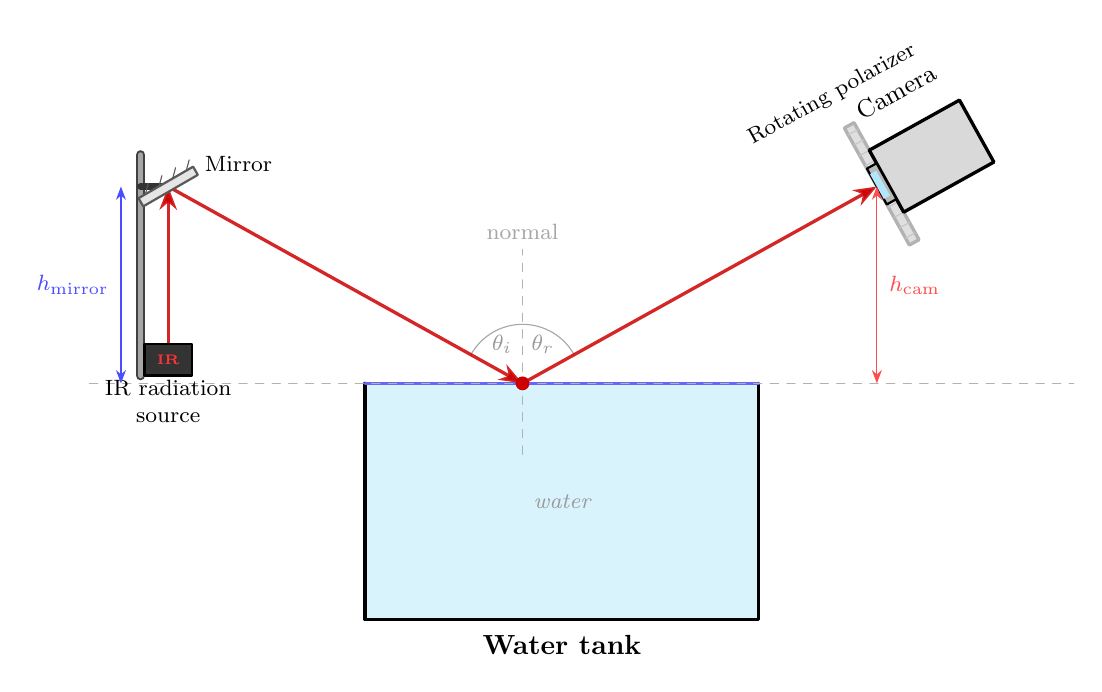
\begin{tikzpicture}[
    >=Stealth,
    line cap=round, line join=round,
    font=\small
]
\def\aqL{0}    \def\aqR{5.0}
\def\aqT{0}    \def\aqB{-3.0}
\def\refX{2.0}
\def\srcX{-2.5}  \def\srcY{2.5}
\def\irY{0.3}
\def\camHgt{2.5}
\def\polX{6.50}   \def\polW{0.14}   \def\polHH{0.85}
\def\camL{6.64}   \def\camR{7.95}   \def\camHH{0.45}
\def\camAngle{29.05}

\fill[cyan!15] (\aqL,\aqB) rectangle (\aqR,\aqT);
\draw[very thick] (\aqL,\aqT) -- (\aqL,\aqB) -- (\aqR,\aqB) -- (\aqR,\aqT);
\draw[very thick, blue!60] (\aqL,\aqT) -- (\aqR,\aqT);
\node[gray!80, font=\footnotesize\itshape] at ({(\aqL+\aqR)/2}, -1.5) {water};
\node[font=\normalsize\bfseries, below=2pt] at ({(\aqL+\aqR)/2}, \aqB) {Water tank};
\draw[gray!60, thin, dashed] (-3.5, 0) -- (9.0, 0);
\draw[gray!60, dashed, thin] (\refX, -0.9) -- (\refX, 1.7)
    node[above, font=\footnotesize, gray!70] {normal};
\draw[gray!70, thin]
    (\refX, 0) ++({90}:0.75)
    arc[start angle=90, end angle=151, radius=0.75];
\node[font=\footnotesize, gray!80] at (\refX-0.26, 0.50) {$\theta_i$};
\draw[gray!70, thin]
    (\refX, 0) ++({29}:0.75)
    arc[start angle=29, end angle=90, radius=0.75];
\node[font=\footnotesize, gray!80] at (\refX+0.26, 0.50) {$\theta_r$};

\draw[->, very thick, red!80!black, opacity=0.85]
    (\srcX, \irY+0.2) -- (\srcX, \srcY);
\draw[->, very thick, red!80!black, opacity=0.85]
    (\srcX, \srcY) -- (\refX, 0);
\draw[->, very thick, red!80!black, opacity=0.85]
    (\refX, 0) -- (\polX, \camHgt);
\fill[red!80!black] (\refX, 0) circle (2.5pt);

\draw[line width=3.5pt, gray!50!black]
    (\srcX-0.35, \irY-0.2) -- (\srcX-0.35, \srcY+0.4);
\draw[line width=2pt, gray!70]
    (\srcX-0.35, \irY-0.2) -- (\srcX-0.35, \srcY+0.4);
\draw[line width=2.5pt, gray!40!black]
    (\srcX-0.35, \srcY) -- (\srcX, \srcY);
\fill[gray!40!black] (\srcX, \srcY) circle (1.5pt);
\node[
    draw,
    fill=black!80,
    thick,
    minimum width=0.6cm,
    minimum height=0.4cm,
    inner sep=0pt,
    text=red!80!white,
    font=\tiny\bfseries
] (IR) at (\srcX, \irY) {IR};
\node[below=4pt, align=center, font=\footnotesize] at (IR) {IR radiation\\source};

\begin{scope}[shift={(\srcX, \srcY)}, rotate=30]
    \fill[gray!20, draw=gray!70!black, thick]
        (-0.4, -0.06) rectangle (0.4, 0.06);
    \foreach \x in {-0.3,-0.1,0.1,0.3} {
        \draw[gray!70!black, thin]
            (\x, 0.06) -- (\x+0.1, 0.16);
    }
\end{scope}
\node[above=8pt, right=4pt, align=center, font=\footnotesize]
    at (\srcX+0.2, \srcY) {Mirror};
\draw[<->, blue!70, thin]
    (\srcX-0.6, 0) -- (\srcX-0.6, \srcY)
    node[midway, left=1pt, blue!70, font=\footnotesize] {$h_{\mathrm{mirror}}$};

\begin{scope}[rotate around={\camAngle:(\polX, \camHgt)}]
\fill[gray!25]
    (\polX, \camHgt-\polHH) rectangle (\polX+\polW, \camHgt+\polHH);
\draw[very thick, gray!60]
    (\polX, \camHgt-\polHH) rectangle (\polX+\polW, \camHgt+\polHH);
\foreach \dy in {-0.75,-0.60,...,0.80}{
    \draw[gray!45, thin]
        (\polX, \camHgt+\dy) -- (\polX+\polW, \camHgt+\dy);
}
\node[
    rotate=\camAngle,
    anchor=south,
    font=\footnotesize,
    align=center
] at (\polX+\polW/2, \camHgt+\polHH+0.2) {Rotating polarizer};
\fill[gray!30]
    (\camL, \camHgt-\camHH) rectangle (\camR, \camHgt+\camHH);
\draw[very thick]
    (\camL, \camHgt-\camHH) rectangle (\camR, \camHgt+\camHH);
\fill[gray!55]
    (\camL-0.14, \camHgt-0.26) rectangle (\camL, \camHgt+0.26);
\draw[thick]
    (\camL-0.14, \camHgt-0.26) rectangle (\camL, \camHgt+0.26);
\fill[cyan!30]
    (\camL-0.14, \camHgt-0.18) rectangle (\camL-0.05, \camHgt+0.18);
\node[rotate=\camAngle, anchor=south]
    at ({(\camL+\camR)/2}, \camHgt+\camHH+0.25) {Camera};
\end{scope}

\draw[<->, red!70, thin]
    (\polX, 0) -- (\polX, \camHgt)
    node[midway, right=1pt, red!70, font=\footnotesize] {$h_{\mathrm{cam}}$};
\end{tikzpicture}%
}
\caption{The experimental measurement setup.}
\label{fig:setup}
\end{figure}

Regarding the measurement itself, five geometries were selected by varying the heights of the camera and the reflecting mirror above the water surface. The projected horizontal distance between the mirror and the pollutant sample in the water tank was kept constant at $d_{\mathrm{mirror}}=70~\mathrm{cm}$, while the camera position was adjusted to maintain the specular observation geometry.

The incidence angle $\theta_i$ of radiation directed from the mirror and the reflection/viewing angle $\theta_r$ toward the imaging system were defined relative to the water-surface normal. Under this specular condition, $\theta_i=\theta_r$ and

\begin{equation}
\theta_i=\tan^{-1}\left(\frac{d_{\mathrm{mirror}}}{h_{\mathrm{mirror}}}\right)=\theta_r,
\end{equation}

\noindent
where $d_{\mathrm{mirror}}$ is the projected horizontal distance between the mirror and the observed sample position. Here, $h_{\mathrm{mirror}}$ is the mirror height above the water surface, and $h_{\mathrm{cam}}$ is the corresponding camera height. All selected experimental geometries used for the measurements are summarized in Table~\ref{tab:measurement_geometry}.

\begin{table}[t]
\centering
\caption{Geometrical configurations used for the multi-angle LWIR polarimetric measurements. The projected mirror distance was fixed at $d_{\mathrm{mirror}}=70~\mathrm{cm}$, and the camera position was adjusted to satisfy the specular condition $\theta_i=\theta_r$. Both angles are defined relative to the water-surface normal.\\}
\label{tab:measurement_geometry}
\begin{tabular}{ccccc}
\toprule
Geometry & $h_{\mathrm{mirror}}$ (cm) & $\theta_i$ ($^\circ$) & $h_{\mathrm{cam}}$ (cm) & $\theta_r$ ($^\circ$) \\
\midrule
G1 & 98.5 & 35.4 & 61 & 35.4 \\
G2 & 76.5 & 42.5 & 49 & 42.5 \\
G3 & 61.0 & 48.9 & 41 & 48.9 \\
G4 & 44.0 & 57.8 & 32 & 57.8 \\
G5 & 31.0 & 66.1 & 23 & 66.1 \\
\bottomrule
\end{tabular}
\end{table}

All microplastic and oil pollutant samples, as well as the water-surface reference, were measured within the same geometry and recorded using the same illumination and observation configuration. To capture the scene at all polarization angles of the rotating polarizer in front of the camera, a video recording was exploited. For each investigated sample, the polarimetric video acquisition consisted of an initial static period of approximately 30~s. In this period the analyzer remained at its home position. This homing procedure was followed by approximately 60~s of continuous analyzer rotation. The angular rotation speed of the analyzer was set to

\begin{equation}
\omega = 20^{\circ}\,\mathrm{s}^{-1}.
\end{equation}

\noindent
The acquired image sequences were stored in the radiometric \texttt{.ravi} video format for subsequent polarization video/image processing.


\subsection{Initial active illumination control measurement}

% Two additional control measurements were performed to provide experimental context for the very low DoLP values obtained from the microplastic samples. First, the water surface was measured three times at an approximately normal observation direction. This measurement was used as an empirical low-polarization reference and was evaluated using the same rotating-analyzer measurement principle.

To assess the overall polarization contribution of the LWIR illumination, an initial measurement with and without active LWIR illumination was conducted. For this purpose, selected members of each pollutant group were exploited. In this case, the water-surface reference (no pollutant), polypropylene (PP), and vegetable oil were evaluated, for simplicity, at three selected measurement geometries ($\text{G}_1, \text{G}_3,\text{G}_5$). For the measurements without active illumination, the optical path from the external LWIR source was physically blocked while the remaining measurement configuration was kept unchanged. 

% These measurements were acquired as a separate control series. Under the blocked-source condition, the weak temporal modulation did not allow a reliable starting phase of the analyzer rotation to be determined. The corresponding AoLP values were therefore not interpreted. The blocked-source DoLP values were retained only as empirical low-response controls and were not used as an instrumental detection limit.


\subsection{Polarization video data processing and statistical analysis}

The obtained radiometric \texttt{.ravi} files from the measurements were converted to raw YUV image sequences using FFmpeg for easier data manipulation before subsequent polarimetric processing. For each captured video sequence, a polygonal region of interest (ROI) corresponding to the investigated sample area was manually selected. The area corresponded to the pixels within the floating wooden ring containing the tested sample. The changing temporal signal was subsequently evaluated from these ROI pixels. For illustration, images of the selected pollutant groups extracted from the obtained video sequences are shown with the highlighted polygonal ROI in Figure~\ref{fig:representative_lwir}.

\begin{figure}[t]
\centering
\begin{minipage}{0.45\textwidth}
\centering
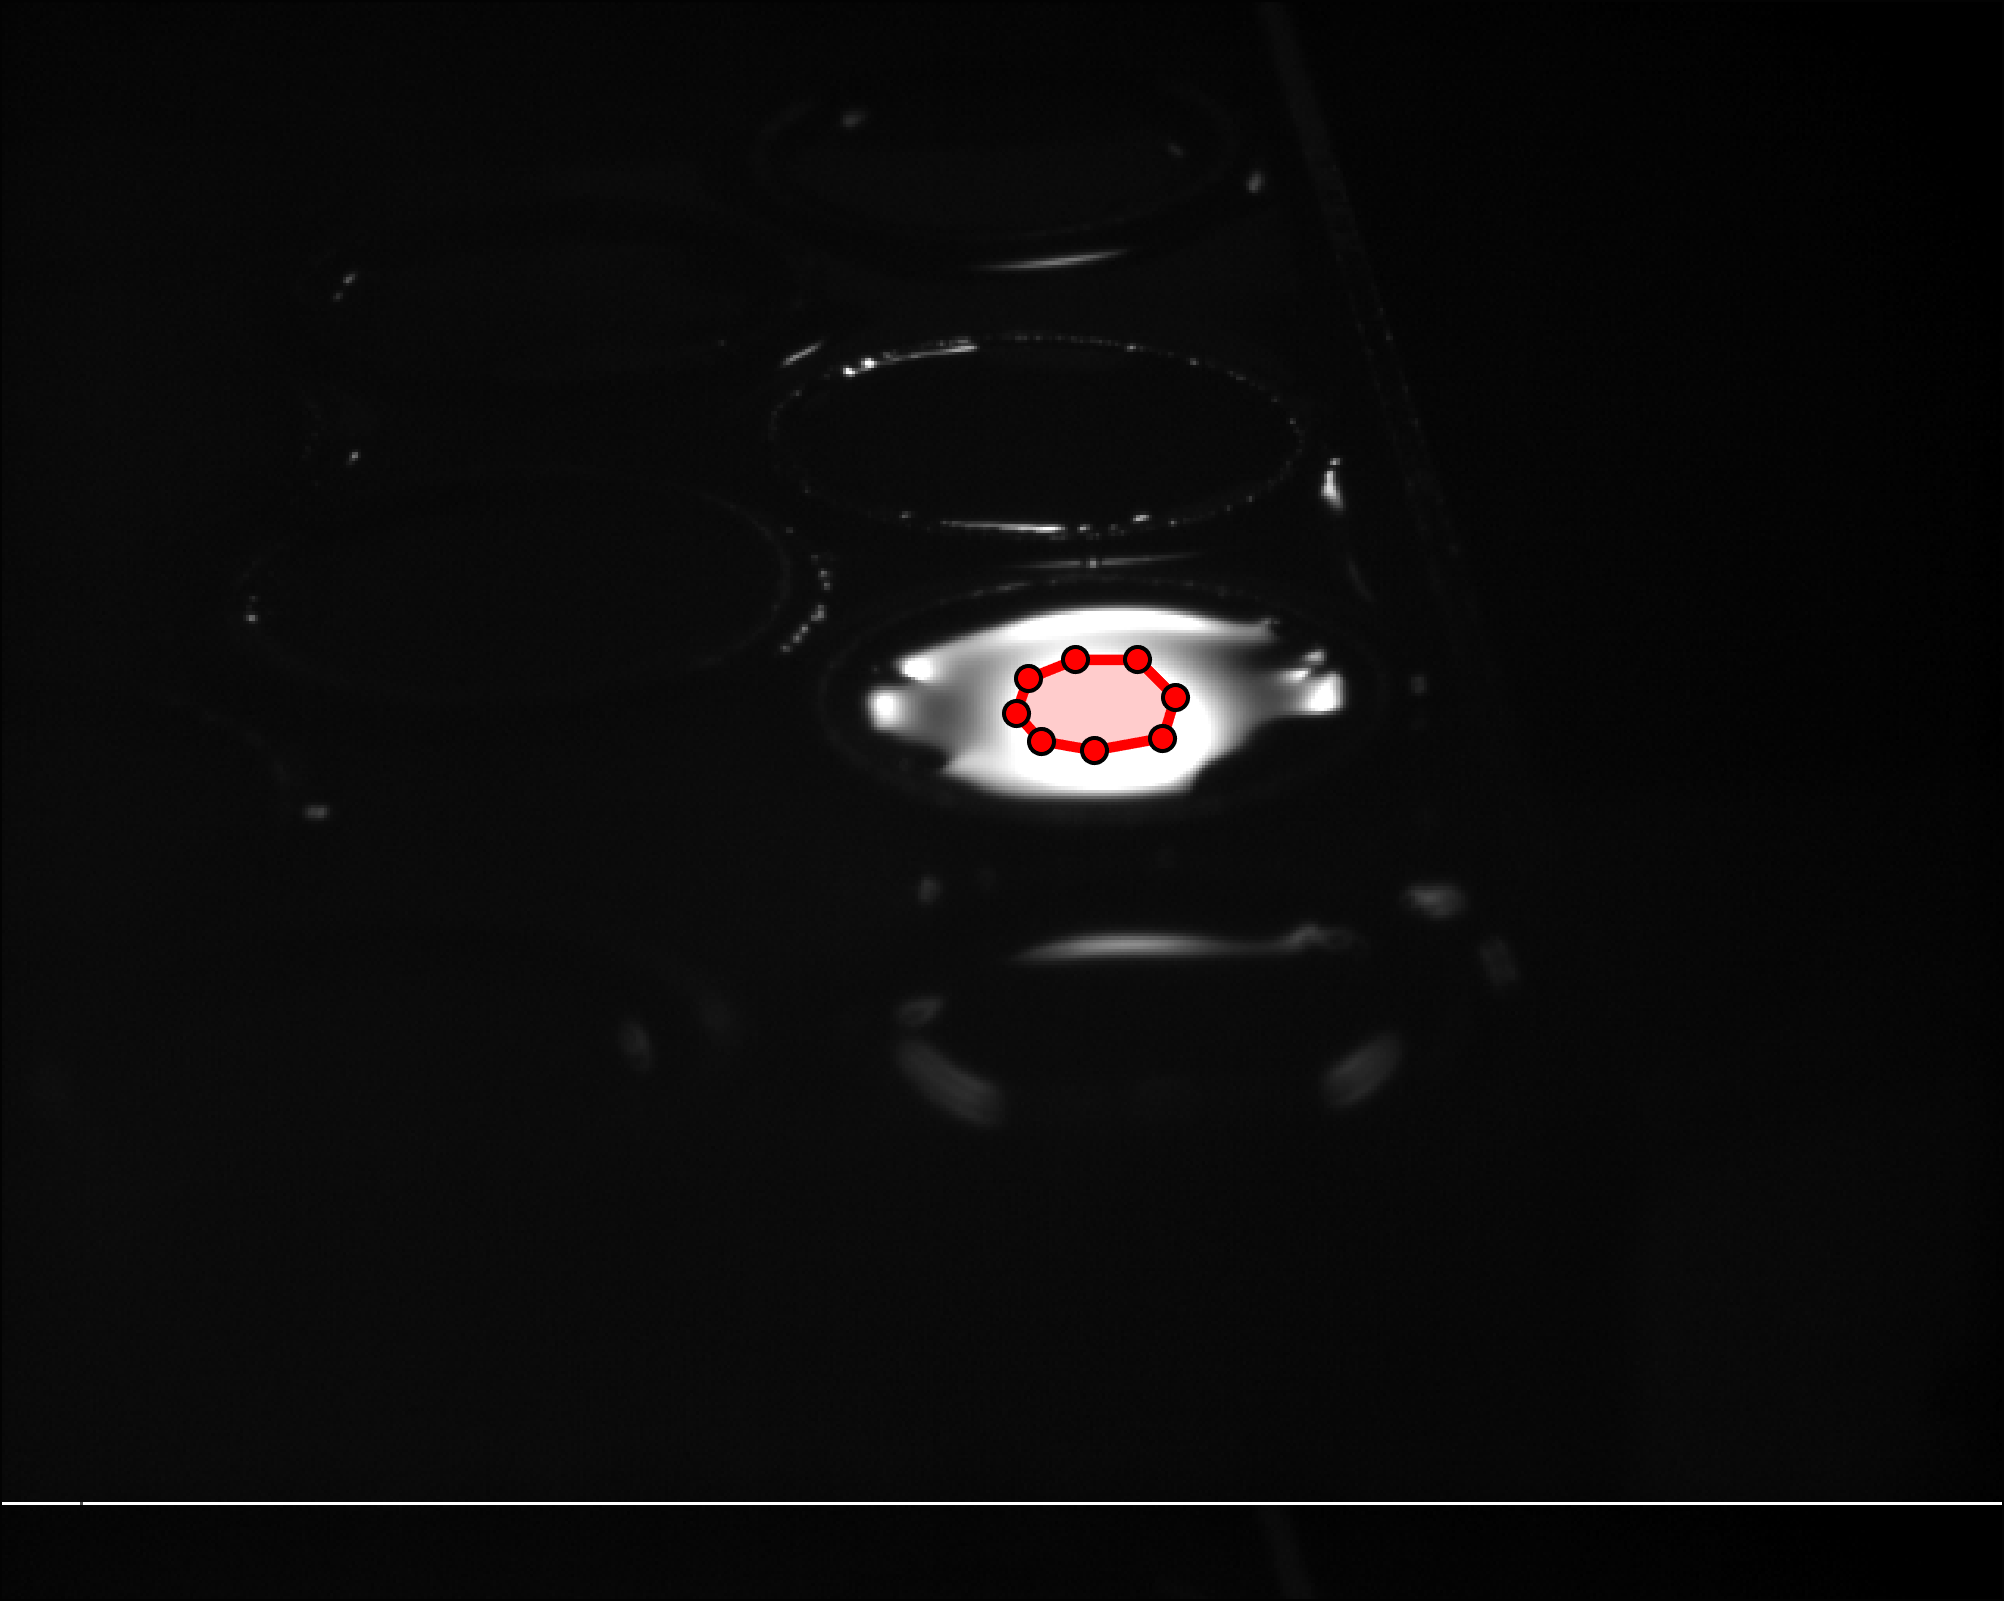
\includegraphics[width=\linewidth]{figures/illustration_with_roi_motor.png}
\par\smallskip{\small\sffamily (a)}
\end{minipage}
\hfill
\begin{minipage}{0.45\textwidth}
\centering
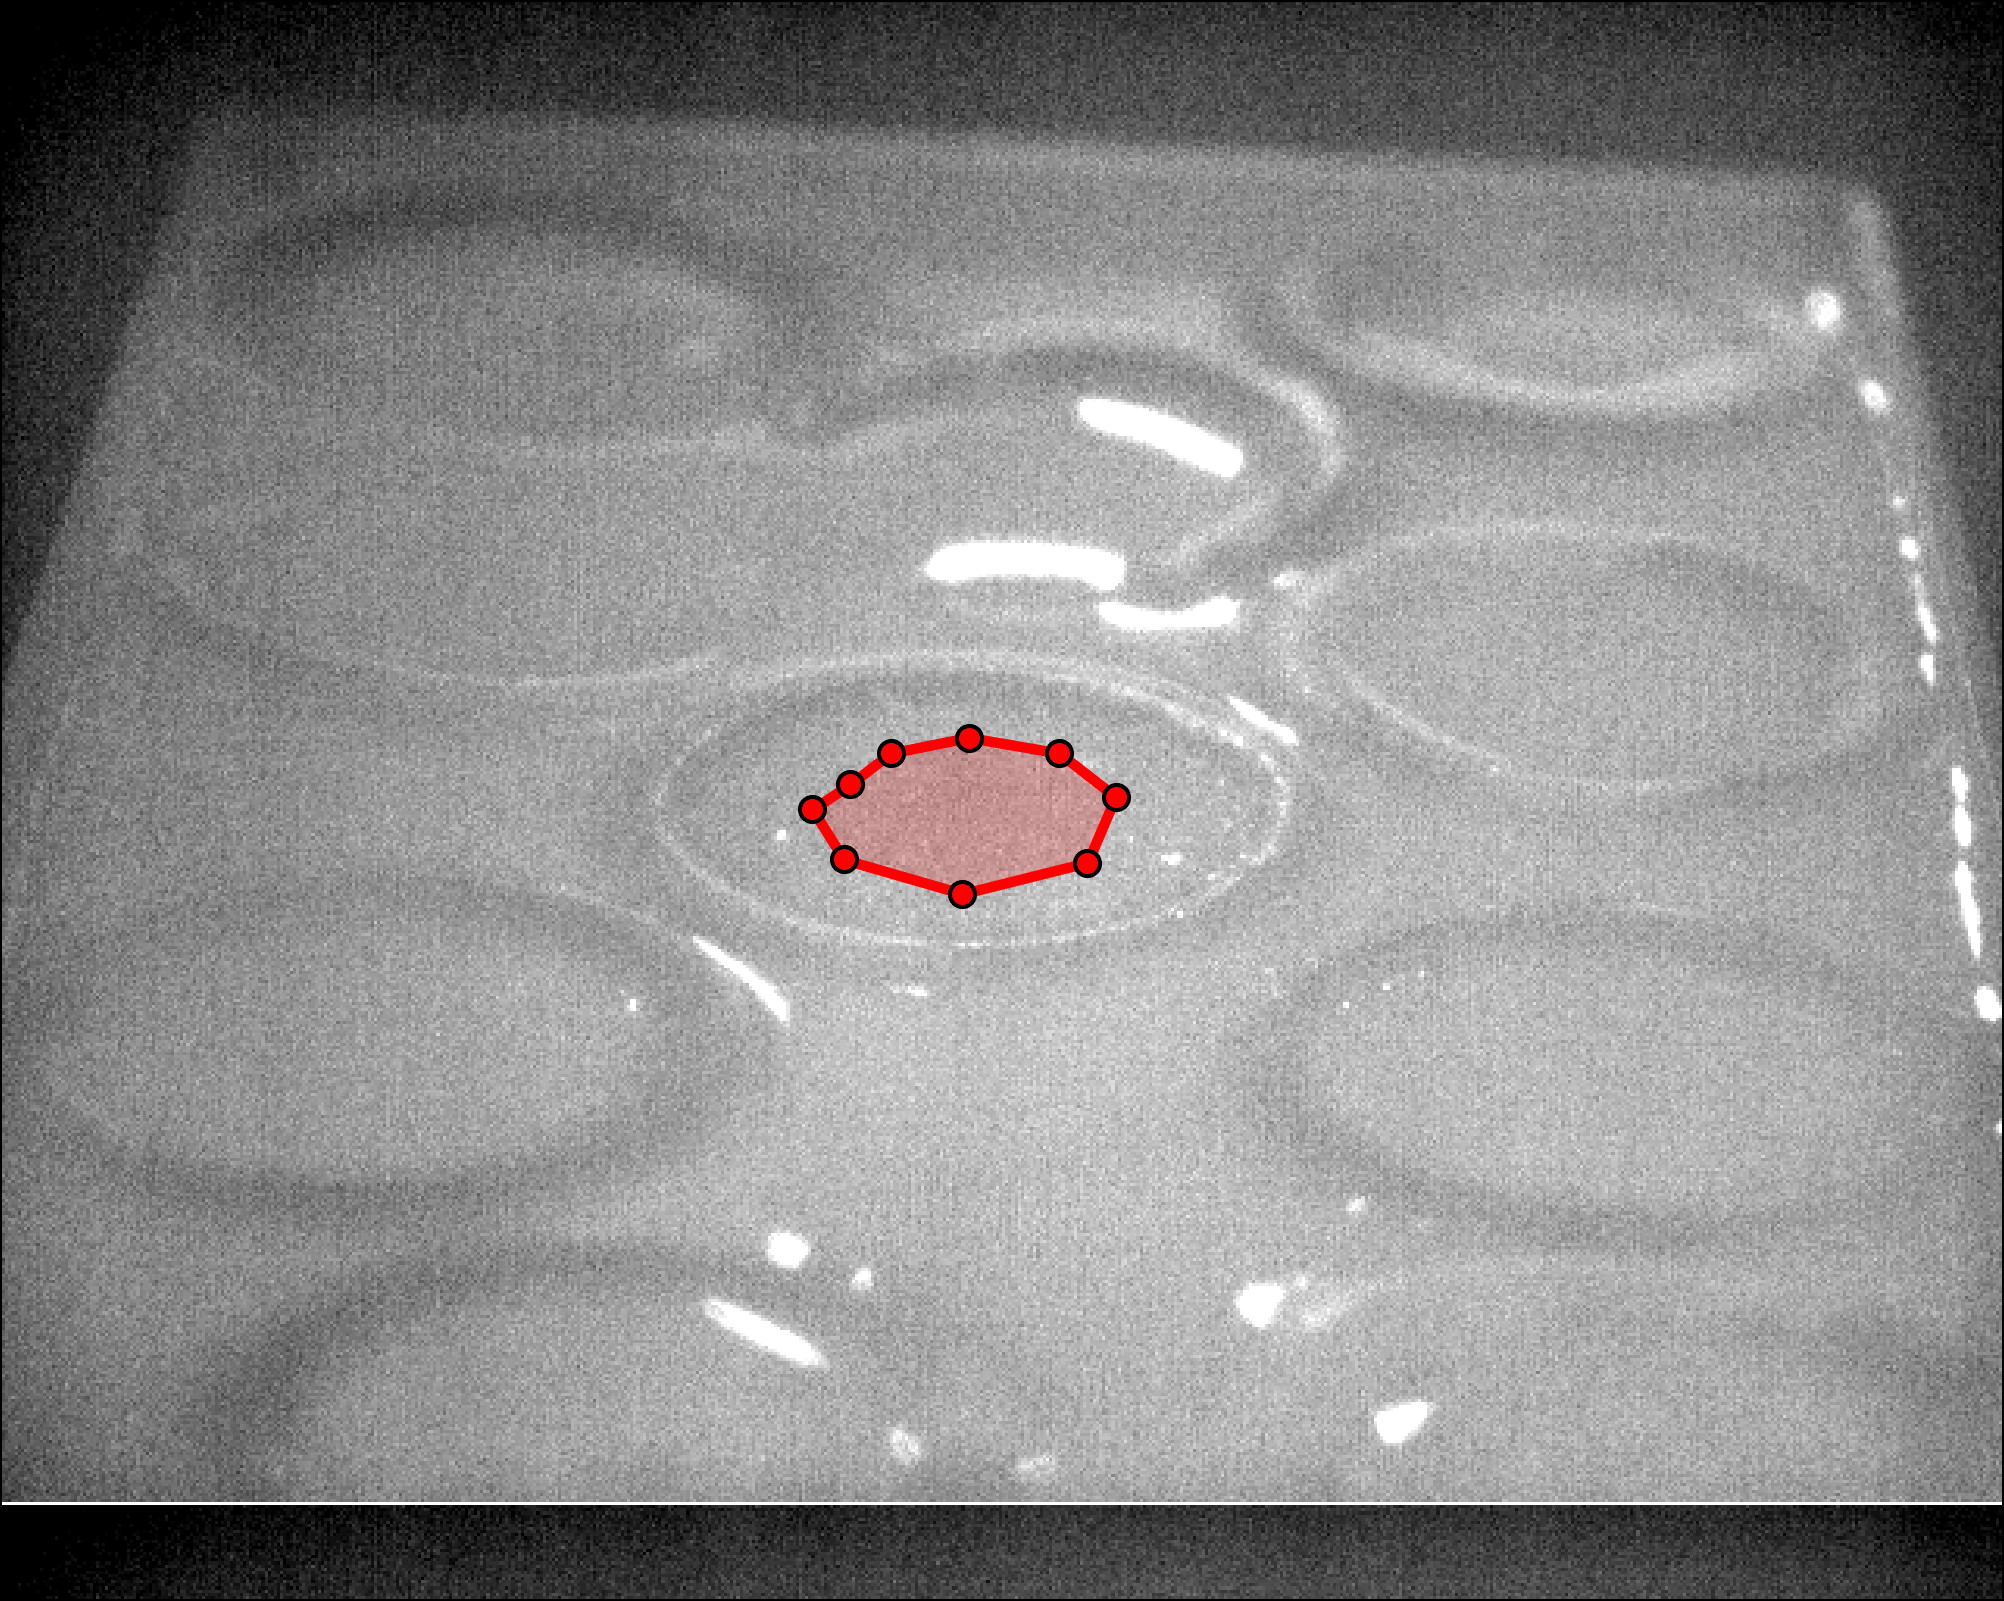
\includegraphics[width=\linewidth]{figures/illustration_with_roi_pcbar.png}
\par\smallskip{\small\sffamily (b)}
\end{minipage}
\caption{Representative LWIR images obtained during the polarimetric measurements. Oil layer (a) and microplastic at the water surface (b). The selected sample polygon ROIs used for polarimetric processing are indicated within both images. The image scale range has been automatically adjusted. Only one wooden ring was used in the same place on the tank for the experimental evaluation. The remaining rings were kept in the water tank to fix the test ring in position. }
\label{fig:representative_lwir}
\end{figure}

Since the video sequences were exploited, the beginning and end of the analyzer rotation were determined from the temporal variation of the mean signal within the selected part of the captured scene. A moving standard deviation with a 5~s window was calculated, and the rotating interval was identified using a threshold corresponding to 25\% of the maximum moving standard deviation. Before each acquisition, the analyzer was initialized at its home position. The image sequence was subsequently restricted to the detected rotating interval, and the first frame of this interval was used as the temporal reference for the subsequent phase calculation.

% In the case of the microplastic samples, the polarization-induced intensity modulation within the particular ROI was substantially weaker. Therefore, a water-reference region visible within the same image sequence was used to determine the analyzer rotation interval and provide a stable phase reference for subsequent harmonic evaluation. This approach enabled the same analyzer phase to be applied to the microplastic ROI even when its temporal modulation was close to the noise level.

Camera calibration (so-called flag) frames or frozen frames that occasionally occurred within the recorded sequences were identified from the temporal signal and excluded before the polarization data evaluation. The original acquisition times of the remaining valid frames were preserved and subsequently used to calculate the corresponding analyzer phase.

Subsequently, each valid pixel within the selected ROI was evaluated independently to retrieve the corresponding linear-polarization parameters (DoLP and AoLP). For a rotating linear analyzer, the measured intensity signal from each pixel contains a second-order angular modulation related to the linear Stokes parameters~\citep{Chipman2018}. For the implemented video processing, the temporal detector signal of each pixel was expressed as

\begin{equation}
 I(t)=A_0+A_2\cos\phi(t)+B_2\sin\phi(t),
 \label{eq:intensity_model}
\end{equation}

\noindent
where $A_0$ is the constant harmonic coefficient, $A_2$ is the cosine coefficient, and $B_2$ is the sine coefficient. The doubled analyzer phase was calculated as

\begin{equation}
 \phi(t)=2\omega t,
 \label{eq:phase}
\end{equation}

\noindent
where $\omega$ denotes the analyzer rotation speed expressed in radians per second and $t$ is the time from the beginning of the detected analyzer rotation interval. For the $k$-th valid frame, $t_k$ corresponds to its original acquisition time within the rotating sequence. 

% Therefore, removal of calibration frames does not alter the analyzer phase assigned to the remaining frames.

For each pixel, the harmonic coefficients were calculated from all $N$ valid frames remaining after calibration-frame removal. The constant component was obtained as the temporal mean

\begin{equation}
 A_0=\frac{1}{N}\sum_{k=1}^{N} I(t_k),
 \label{eq:A0}
\end{equation}

\noindent
while the cosine and sine components were determined by discrete harmonic projection according to

\begin{equation}
 A_2 = \frac{2}{N}\sum_{k=1}^{N}\left[I(t_k)-A_0\right]\cos\phi_k,
\end{equation}

\noindent
and
\begin{equation} 
 B_2 = \frac{2}{N}\sum_{k=1}^{N}\left[I(t_k)-A_0\right]\sin\phi_k,
 \label{eq:harmonic_coefficients}
\end{equation}

\noindent
where $\phi_k=\phi(t_k)$ is the doubled analyzer phase corresponding to the $k$-th valid frame. The first three Stokes parameters~\citep{Schaefer2007} were subsequently calculated as

\begin{align}
 S_0 &= 2A_0, \\
 S_1 &= 2A_2, \\
 S_2 &= 2B_2.
 \label{eq:stokes}
\end{align}

\noindent
Only linear polarization parameters were evaluated in the experiment. Thus, the circular Stokes component $S_3$ was omitted. The degree of linear polarization was calculated as

\begin{equation}
 \mathrm{DoLP}=\frac{\sqrt{S_1^2+S_2^2}}{S_0},
 \label{eq:dolp}
\end{equation}

\noindent
and the angle of linear polarization as

\begin{equation}
 \mathrm{AoLP}=\frac{1}{2}\operatorname{atan2}(S_2,S_1).
 \label{eq:aolp}
\end{equation}

The resulting AoLP values were expressed in degrees and mapped to the interval $[-90^{\circ},90^{\circ}]$.

For each ROI, the pixel-wise DoLP distribution was initially characterized by its arithmetic mean $\mu_D$ and standard deviation $\sigma_D$. Pixels fulfilling
\begin{equation}
 \left|\mathrm{DoLP}_k-\mu_D\right|>3\sigma_D
\end{equation}

or providing non-physical values with $\mathrm{DoLP}_k>1$ were excluded from the subsequent regional evaluation. The final DoLP value of each ROI was calculated as the arithmetic mean of the remaining valid pixel values, and their standard deviation was used to characterize the DoLP variability within the ROI.

Since the orientation of linear polarization is an axial quantity with a periodicity of 180$^{\circ}$, the AoLP values were evaluated using doubled-angle circular statistics. For the $N_p$ valid pixel angles $\alpha_k$, the mean Cartesian components were calculated as

\begin{equation}\label{eq:circular_xy}
 X = \frac{1}{N_p}\sum_{k=1}^{N_p}\cos(2\alpha_k), 
\end{equation}
\begin{equation}
 Y = \frac{1}{N_p}\sum_{k=1}^{N_p}\sin(2\alpha_k),
\end{equation}

\noindent
and the regional mean AoLP was obtained as

\begin{equation}
 \bar{\alpha}=\frac{1}{2}\operatorname{atan2}(Y,X).
 \label{eq:circular_mean}
\end{equation}

\noindent
The corresponding mean resultant length was calculated as

\begin{equation}
 R=\sqrt{X^2+Y^2},
 \label{eq:resultant_length}
\end{equation}

\noindent
and the axial circular standard deviation as

\begin{equation}
 \sigma_{\alpha}=\frac{1}{2}\sqrt{-2\ln R}.
 \label{eq:circular_std}
\end{equation}

\noindent
The circular calculations were performed in radians and the resulting mean AoLP and standard deviation were subsequently converted to degrees.

For the direct final comparison of the two pollutant groups (microplastics and oils), the mean ROI DoLP values of the individual materials were combined separately for the microplastic and oil samples. The calculations were performed independently for each discrete measurement geometry $g\in\{\mathrm{G1},\ldots,\mathrm{G5}\}$. The DoLP response of each pollutant group was summarized using the following root-mean-square equation

\begin{equation}
 D_{\mathrm{RMS},c}(g)=
 \sqrt{\frac{1}{N_c}\sum_{i=1}^{N_c}\bar{D}_{i}^{\,2}(g)},
 \label{eq:rms_dolp}
\end{equation}

\noindent
where $c$ denotes the investigated pollutant group, $N_c$ is the number of tested materials within the group, and $\bar{D}_{i}(g)$ is the mean ROI DoLP of the $i$-th material at geometry $g$. To account for both the spatial variability within the individual ROIs and the spread among the tested materials, the total standard deviation for each pollutant group was evaluated using the law of total variance as

\begin{equation}
 \sigma_{\mathrm{total},c}(g)=
 \sqrt{
 \frac{1}{N_c} \sum_{i=1}^{N_c} \sigma_{i}^2(g) +
 \frac{1}{N_c-1}
 \sum_{i=1}^{N_c}
 \left[\bar{D}_{i}(g)-\mu_c(g)\right]^2},
 \label{eq:class_sd}
\end{equation}

\noindent
where $\mu_c(g)$ is the arithmetic mean of the DoLP values obtained for the individual materials within the corresponding group, and $\sigma_i(g)$ is the pixel-level standard deviation within the ROI of the $i$-th material. The obtained RMS values and the associated total standard deviation were used as descriptive measures of the polarization response and overall variability within each pollutant group.

For the comparison of AoLP between the two pollutant groups, the mean AoLP values obtained for the individual materials were combined using the same doubled-angle circular statistics defined in Equations~\eqref{eq:circular_xy}--\eqref{eq:circular_std}. This approach preserves the axial character of the polarization orientation and avoids direct linear or RMS averaging of angular quantities.

% ------------------------------------------------------------------

\section{Experimental results}
% ------------------------------------------------------------------

\subsection{Initial active illumination control measurements}

% The additional water-surface control measured at an approximately normal observation direction provided very low DoLP values. The three measurements yielded mean DoLP values of $2.5\times10^{-4}$, $4.4\times10^{-4}$, and $5.6\times10^{-4}$. Thus, the empirical low-polarization reference remained within the order of $10^{-4}$. These values provide experimental context for the low DoLP obtained from the microplastic samples and are not interpreted as an instrumental detection limit.

The measurements with and without active LWIR illumination provided a direct comparison of the contribution of the illumination source. The results of the DoLP analysis are presented in Figure~\ref{fig:active_illumination_control}. With active illumination, the DoLP of water ranged from $8.36\times10^{-3}$ to $3.81\times10^{-2}$. With the external source blocked, the water values remained between $4.30\times10^{-4}$ and $5.20\times10^{-4}$ and were therefore significantly lower. For vegetable oil, the DoLP ranged from $9.94\times10^{-3}$ to $6.25\times10^{-2}$ with active illumination and from $2.30\times10^{-4}$ to $5.40\times10^{-4}$ with the source blocked. The PP response remained within the same order under both conditions. Its DoLP ranged from $2.00\times10^{-4}$ to $4.80\times10^{-4}$ with active illumination and from $2.90\times10^{-4}$ to $4.50\times10^{-4}$ with the source blocked. Therefore, it is clear that active illumination produced a substantially higher DoLP response for the water-surface reference and vegetable oil, while no comparable increase was observed for PP. The corresponding Stokes coefficients showed that this change was mainly associated with the magnitude of the linear polarization components, $\sqrt{S_1^2+S_2^2}$, while the variation in $S_0$ was considerably smaller. In the case of the AoLP analysis with a blocked illumination path, the DoLP was so low that a reliable interpretation of the AoLP values was not possible. Thus, the AoLP graphical output for this measurement was excluded from the results. 

\begin{figure}[t]
\centering
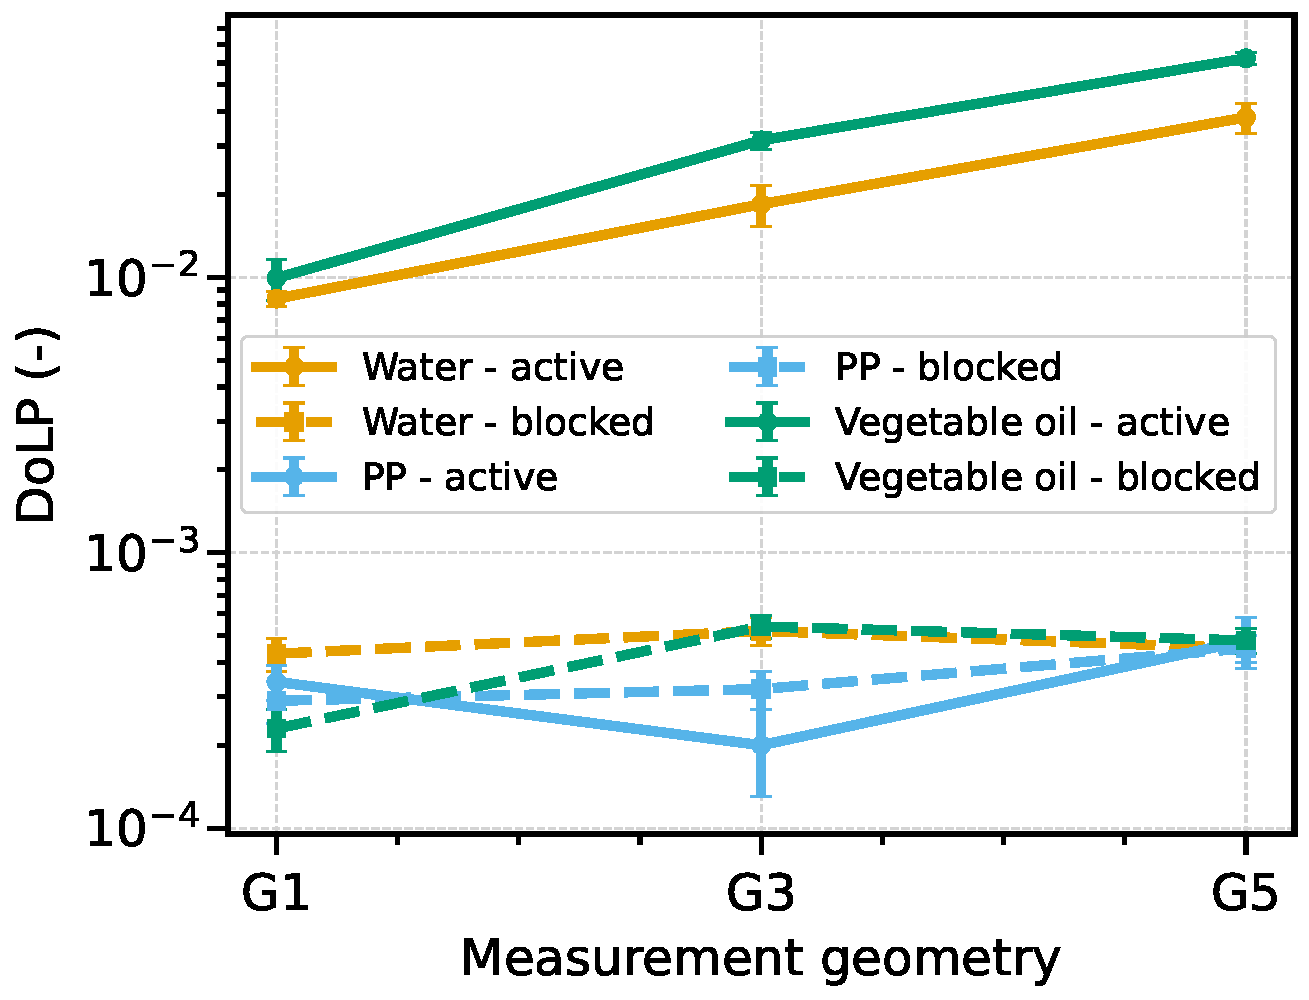
\includegraphics[width=0.55\textwidth]{figures/active_illumination_control_DOLP.pdf}
\caption{Comparison of DoLP obtained for water-surface reference, polypropylene (PP), and vegetable oil with active LWIR illumination and with the external source blocked at measurement geometries G1, G3, and G5. Error bars indicate the variability of each ROI measurement.}
\label{fig:active_illumination_control}
\end{figure}

\subsection{Variability among the investigated pollutant samples}

The complete microplastic set exhibited very low DoLP values. The results can be seen in Figure~\ref{fig:all_dolp}. Across all nine investigated plastic materials and five measurement geometries, the mean DoLP of the individual materials ranged from $1.80\times10^{-4}$ to $1.10\times10^{-3}$, while the values varied among the materials. No common monotonic dependence on measurement geometry was observed for the complete microplastic set.

\begin{figure}[t]
\centering
\begin{minipage}{0.48\textwidth}
\centering
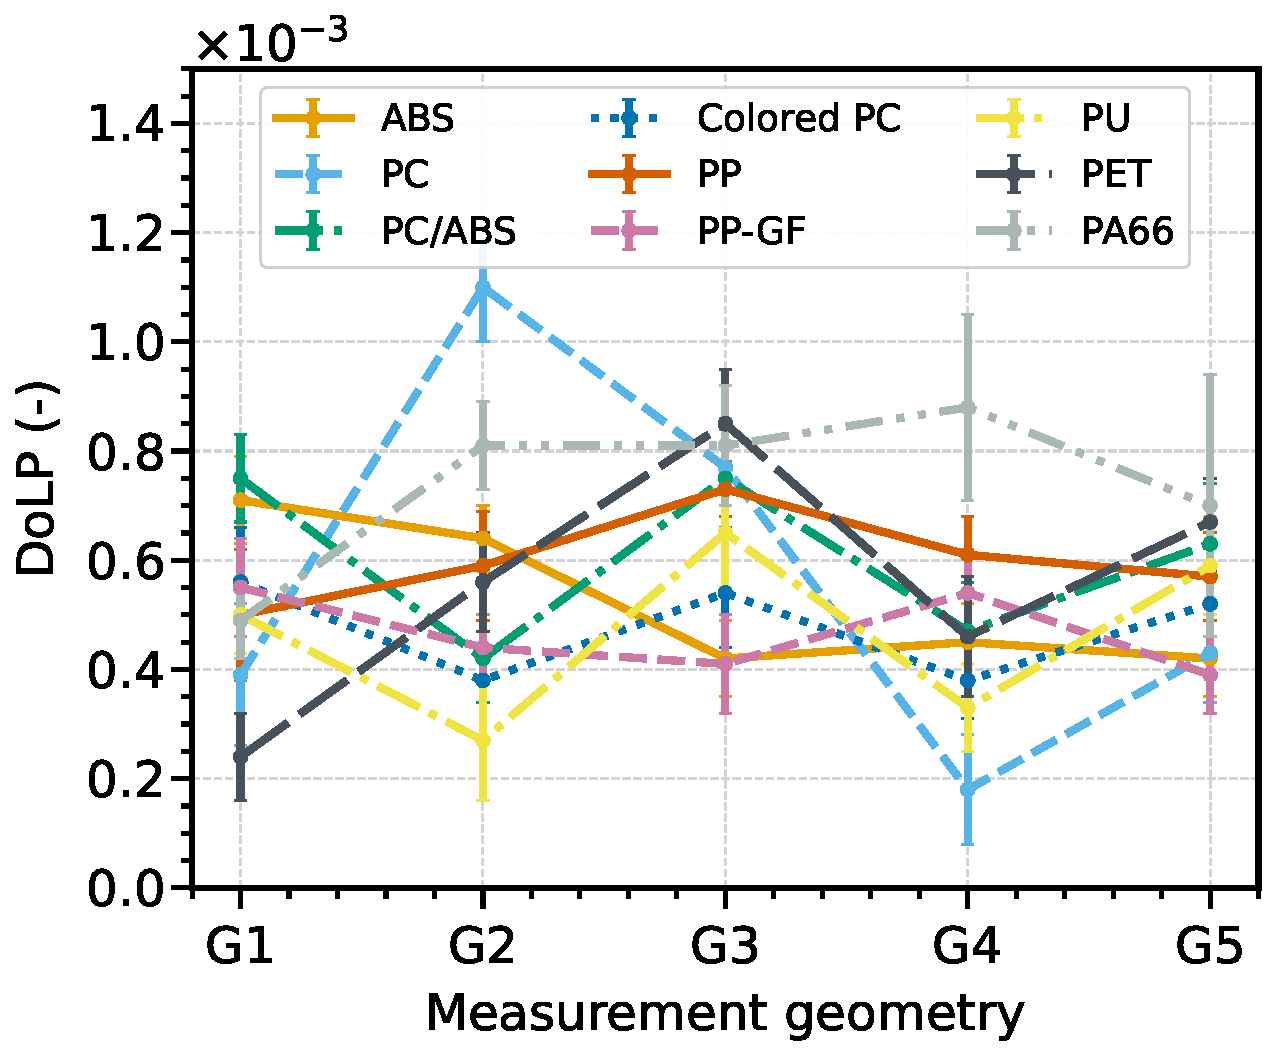
\includegraphics[width=\linewidth]{figures/03_all_microplastics_DOLP.pdf}
\par\smallskip{\small\sffamily (a)}
\end{minipage}
\hfill
\begin{minipage}{0.48\textwidth}
\centering
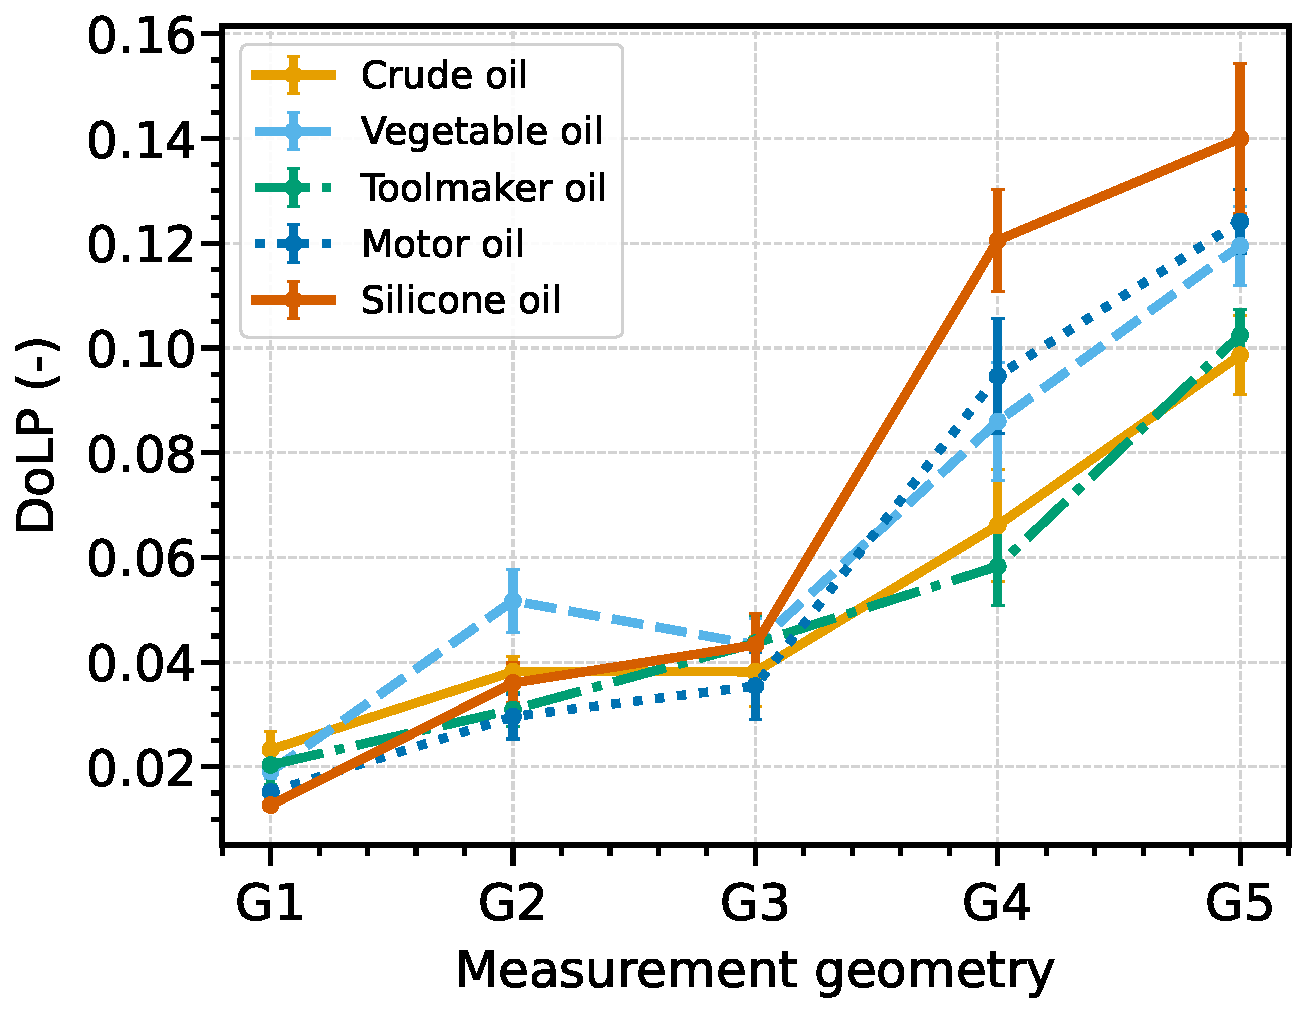
\includegraphics[width=\linewidth]{figures/05_all_oils_DOLP.pdf}
\par\smallskip{\small\sffamily (b)}
\end{minipage}
\caption{DoLP characteristics of all investigated microplastic samples at the water surface (a) and oil samples (b) across the five measurement geometries.}
\label{fig:all_dolp}
\end{figure}

The oil samples exhibited substantially higher DoLP values. The mean values of the individual oils were within the range from $1.27\times10^{-2}$ to $1.40\times10^{-1}$. In general, the oil response increased toward the more oblique measurement geometries, although the detailed angular response differed among the oils. Crude oil showed a less monotonic dependence than several of the other oil samples.

The most consistent result was obtained in the comparison of the individual materials against the water-surface reference. For every measurement geometry, the DoLP of all nine microplastic materials remained below the mean DoLP of water. In contrast, the DoLP of all five oil samples remained above the water reference. Therefore, the DoLP ranges of the investigated microplastic and oil samples did not overlap under the laboratory conditions used in this experiment.

By contrast, the AoLP characteristics of the materials varied more, especially for the microplastic samples, which was expected due to the low levels of DoLP. Individual microplastics exhibited a significant range of AoLP values from $-20^{\circ}$ to above $40^{\circ}$ and varied across the measurement geometry set (see Figure~\ref{fig:all_aolp}). The oil AoLP values were generally concentrated within a narrower angular interval from $-2.5^{\circ}$ to above $12.5^{\circ}$. 
% The water-surface sample varied around an AoLP of $-60^{\circ}$, which was distinct from the pollutant ranges. 

\begin{figure}[t]
\centering
\begin{minipage}{0.48\textwidth}
\centering
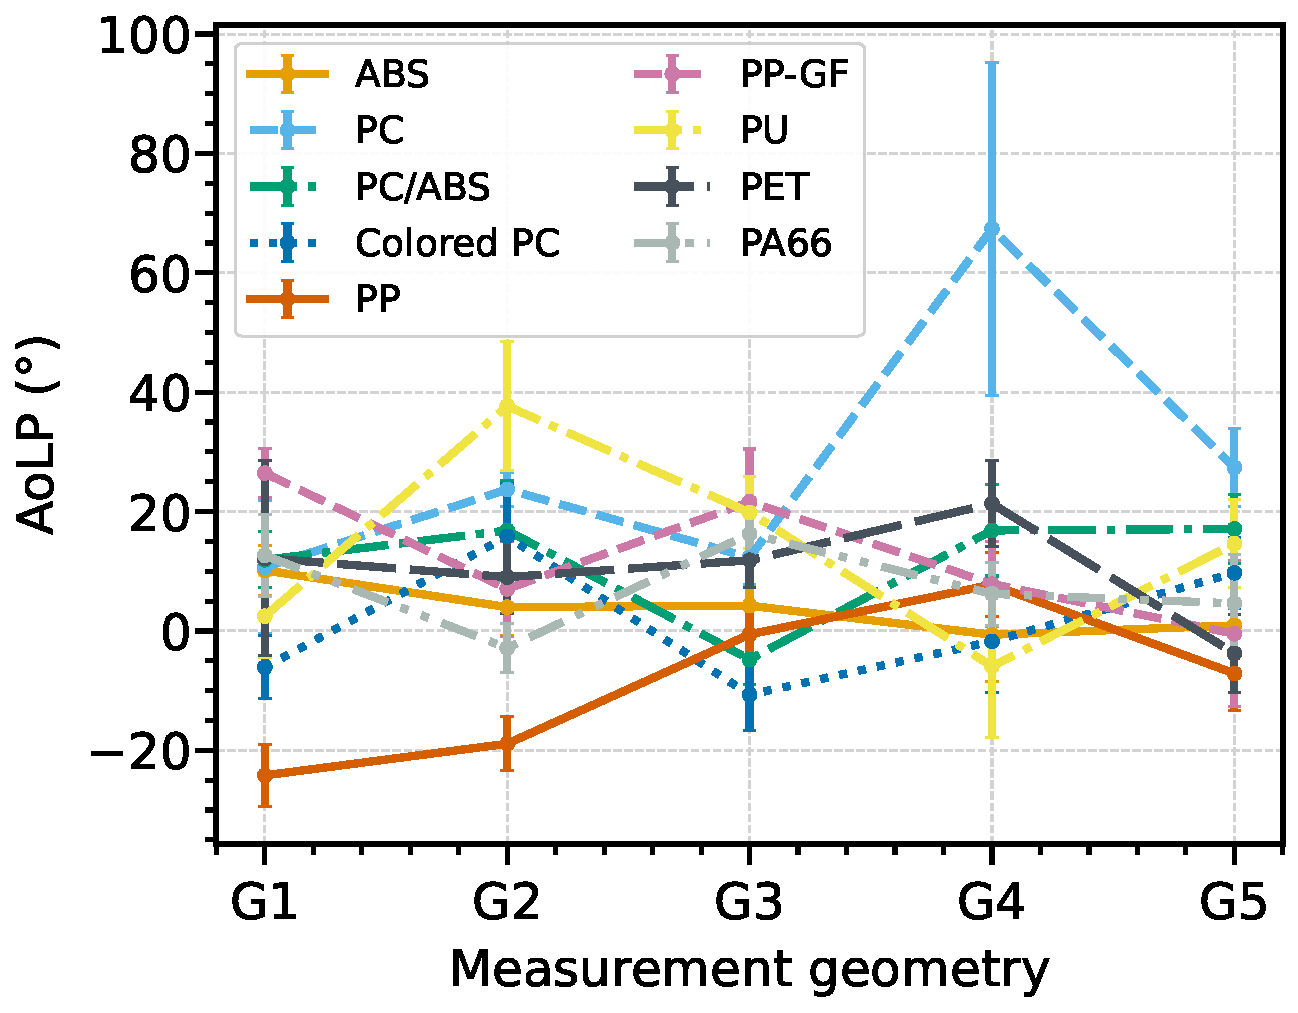
\includegraphics[width=\linewidth]{figures/04_all_microplastics_AOLP.pdf}
\par\smallskip{\small\sffamily (a)}
\end{minipage}
\hfill
\begin{minipage}{0.48\textwidth}
\centering
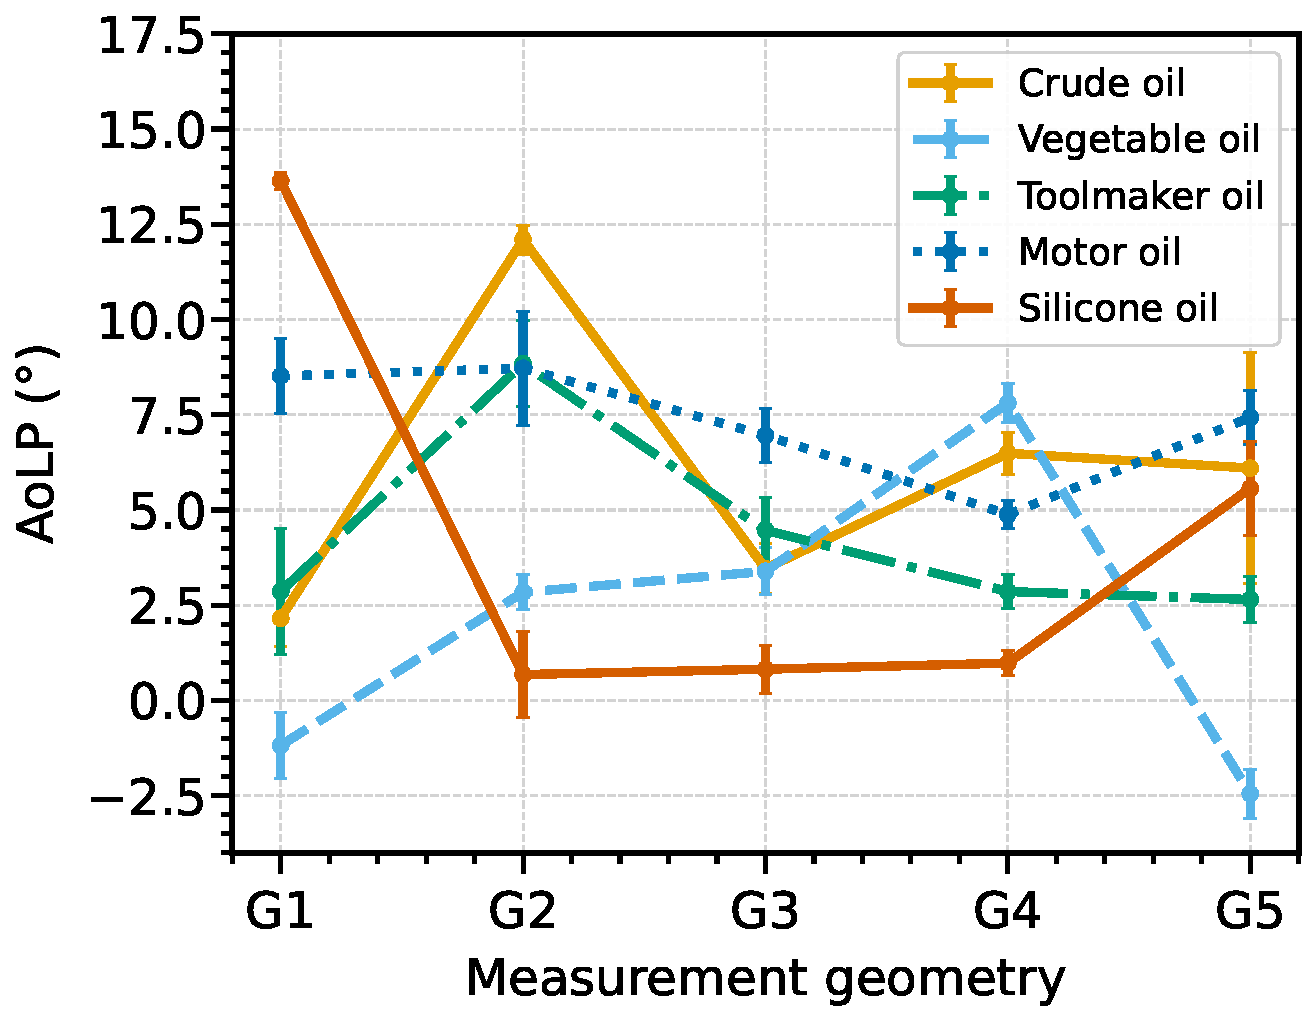
\includegraphics[width=\linewidth]{figures/06_all_oils_AOLP.pdf}
\par\smallskip{\small\sffamily (b)}
\end{minipage}
\caption{AoLP characteristics of all investigated microplastic samples at the water surface (a) and oil samples (b) across the five measurement geometries.}
\label{fig:all_aolp}
\end{figure}



\subsection{Comparison of the microplastic and oil sample groups}

The pollutant group comparison confirms the substantial
difference in DoLP (Figure~\ref{fig:class_comparison}). The RMS DoLP of the nine microplastic materials remained within the range $5.12\times10^{-4}$--$6.77\times10^{-4}$ across all five measurement geometries. The RMS DoLP of the five oil samples was significantly higher and increased from $1.85\times10^{-2}$ in G1 up to $1.18\times10^{-1}$ in G5.

The mean DoLP of the water reference remained between the two pollutant groups across all investigated geometries. It increased from $3.29\times10^{-3}$ in G1 to $4.49\times10^{-2}$ in G5. The water-surface reference therefore remained above the microplastic RMS DoLP and below the oil RMS DoLP throughout all angular measurements. This ordering was consistent across all materials and geometries.

\begin{figure}[t]
\centering
\begin{minipage}{0.48\textwidth}
\centering
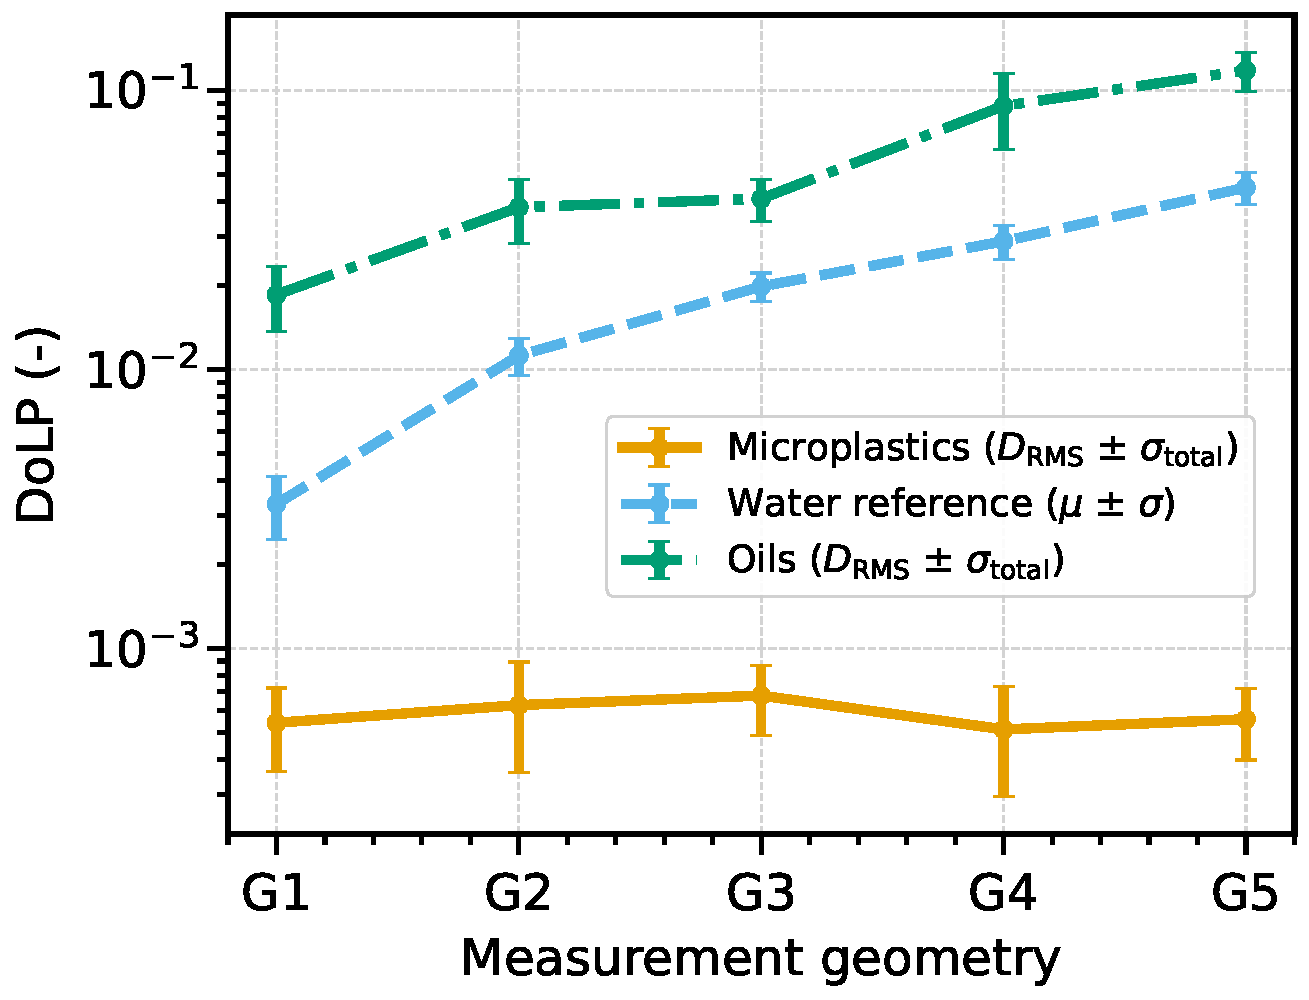
\includegraphics[width=\linewidth]{figures/07_class_DOLP_with_water.pdf}
\par\smallskip{\small\sffamily (a)}
\end{minipage}
\hfill
\begin{minipage}{0.48\textwidth}
\centering
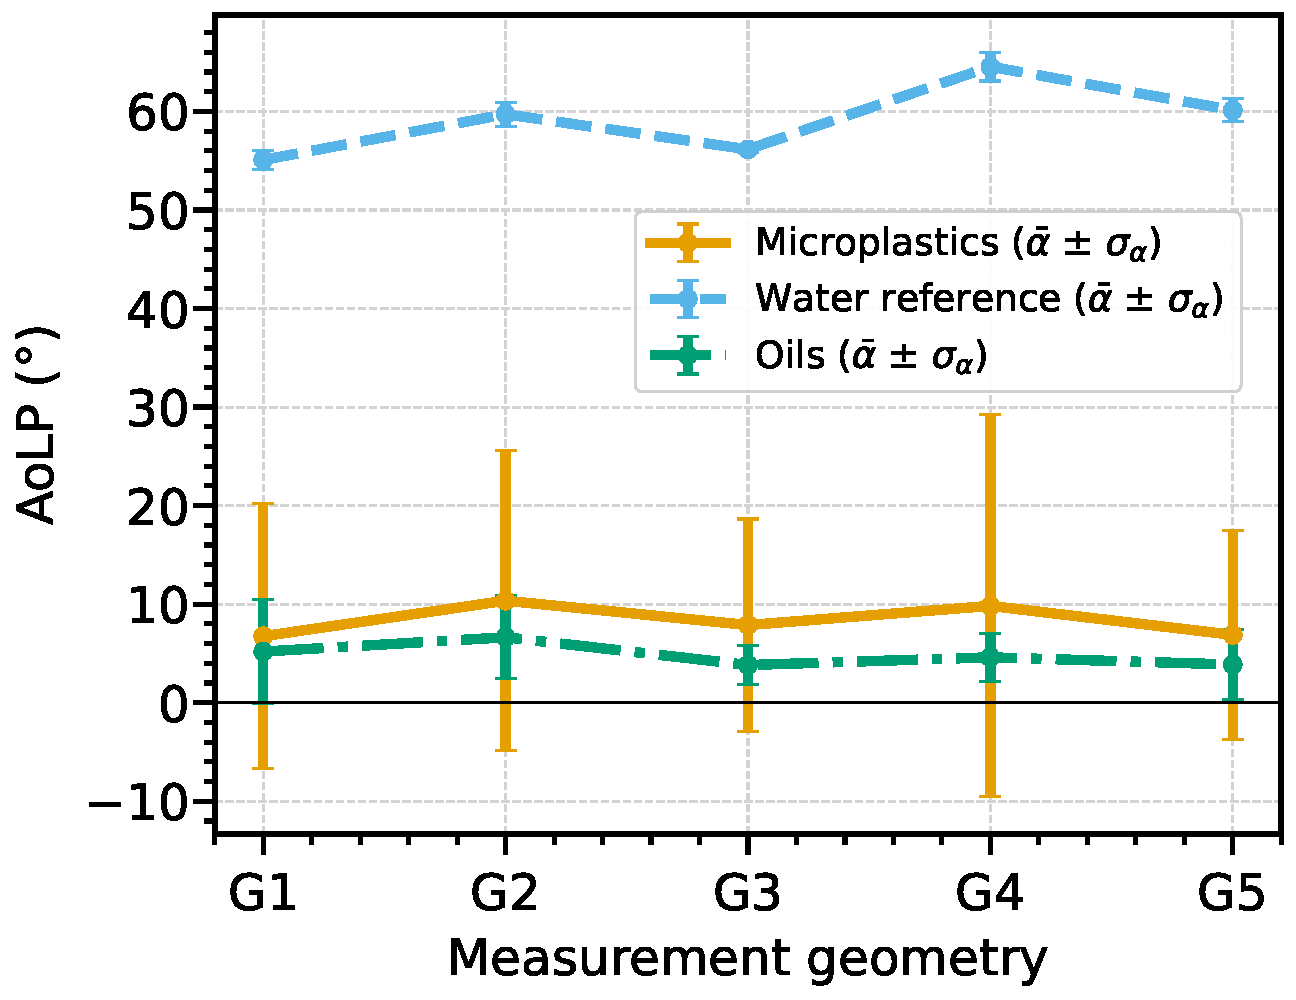
\includegraphics[width=\linewidth]{figures/08_class_AOLP_circular.pdf}
\par\smallskip{\small\sffamily (b)}
\end{minipage}
\caption{Comparison of the investigated pollutant groups. (a): RMS DoLP of the microplastic and oil groups together with the mean DoLP of the water-surface reference. Error bars for the pollutant groups represent the total standard deviation defined in Eq.~\eqref{eq:class_sd}. (b): mean AoLP of the pollutant groups calculated using doubled-angle circular statistics; error bars represent the corresponding circular standard deviation.}
\label{fig:class_comparison}
\end{figure}

The mean AoLP characteristics did not show a comparable separation between pollutants (Figure~\ref{fig:class_comparison}). The circular mean AoLP of the microplastic group ranged from approximately 6.7$^{\circ}$ to 10.4$^{\circ}$, while the oil group ranged from approximately 3.8$^{\circ}$ to 6.6$^{\circ}$. The circular standard deviation was approximately 10.6$^{\circ}$--19.4$^{\circ}$ for the microplastic group and 2.0$^{\circ}$--5.3$^{\circ}$ for the oil group. The water-surface sample varied around an AoLP of $60^{\circ}$, which was, however, distinct from the pollutant ranges. 

In general, the main difference between the groups of investigated pollutants was related to the magnitude of linear polarization. It was observed that AoLP provided substantially weaker separation. However, as previously mentioned, the water AoLP results suggested the potential to distinguish the water surface from the pollutants, though further investigation is necessary.

% ------------------------------------------------------------------

\section{Discussion}
% ------------------------------------------------------------------

The main experimental result showed a consistent difference in DoLP between the pollutant groups and the water-surface reference. The microplastics exhibited a very low DoLP response. The water-surface reference provided an intermediate response, and the prepared oil layers showed the highest DoLP values. This ordering was observed for all five measurement geometries. Under the present laboratory conditions, DoLP therefore distinguished the investigated microplastics from the oils and from the water-surface reference more clearly than AoLP.

In addition, the control measurements provide important context. Water and vegetable oil showed substantially higher DoLP with active LWIR illumination than with the blocked illumination path. PP remained within the same very low DoLP range under both illumination conditions. 
Evaluation of the corresponding Stokes coefficients showed that the reduction in DoLP after blocking the external source was mainly associated with a decrease in the magnitude of the linear polarization components, $\sqrt{S_1^2+S_2^2}$. Moreover, the change in $S_0$ was considerably smaller for water and vegetable oil. This supports the interpretation that the observed DoLP difference was primarily related to the polarization effects rather than to a change in the overall intensity level.
The observed dependence on illumination is consistent with the known sensitivity of LWIR polarimetric signatures to the radiative state of the target and its optical background~\citep{Tyo2007}. The blocked-source measurements were used only as empirical low-response controls since the weak polarization effect did not provide a reliable phase reference for the AoLP interpretation.

The response of the water surface is also important for interpretation of the pollutant measurements. Thermal radiation from water is known to exhibit a polarization response that changes with observation geometry~\citep{Shaw1999,Shaw2001}. In the present experiment, the DoLP of the water reference increased toward the more oblique geometries. A higher polarization response of the oil samples is also consistent with previous theoretical and experimental studies of thermal polarization from oil-covered water surfaces~\citep{Zhang2014,Chenault2018,Fu2022,Sun2023}. The results of the paper extend the comparison by measuring oils, microplastics, and the water-surface reference using the same experimental geometry.

It is apparent that the microplastics behaved differently in terms of polarization. Their DoLP remained very low and did not exhibit a common monotonic increase with measurement geometry. Therefore, the measured polarization response should be interpreted as a property of the complete particle--water-surface scene rather than as an intrinsic polarization property of an individual polymer. This distinction is important. Published thermal infrared measurements show that plastic litter can exhibit diagnostic LWIR spectral features~\citep{Garaba2020}, but those spectral results do not directly define the polarization response of particles distributed at a water surface. Several effects may contribute to the low measured DoLP, including particle shape and surface roughness, particle orientation and packing, the fraction of exposed water within the ROI, and multiple reflection or scattering at the particle--water--air interfaces. The presented experiment was not designed to separate and investigate these effects. Accordingly, small differences among the tested plastic materials should not be interpreted as validated polarization signatures of individual polymers. Therefore, the subsequent analysis is required.

The individual oils also showed different angular DoLP characteristics. The gradient and detailed shape of the DoLP curves varied among the investigated oil types. These differences may contain information related to the physical and optical properties of the oils, but the present dataset is not sufficient for oil-type identification. The nominal thicknesses of the prepared oil layers ranged from 2.57 to 4.05~mm. The obtained results therefore apply to these millimeter-scale laboratory layers and should not be extrapolated directly to thin environmental oil spills. For this purpose, further detailed investigation is necessary, and a systematic evaluation of oil-layer thickness would be required before such an extrapolation could be made.

The AoLP parameter provided complementary information but did not show the same distinction between the pollutant groups. The average AoLP values of the groups substantially overlapped, and the microplastic samples showed considerably greater angular dispersion. In addition, the absolute AoLP orientation depends on the adopted analyzer phase reference, which was not independently calibrated in the experiment. The absolute AoLP values should therefore be interpreted cautiously. The results support DoLP as the more informative parameter for comparison of the investigated water-surface conditions.

Several additional limitations should be considered when interpreting the environmental relevance of the results. The measurements were performed under active LWIR illumination using fresh tap water and a comparatively stable water surface. The floating-ring configuration confined the prepared microplastic materials to a defined surface region and should be considered as a controlled surface condition rather than a representation of natural particle abundance or spatial distribution. However, natural aquatic environments introduce additional effects related to water temperature and salinity, wind-induced surface roughness, waves, ageing of microplastics, spreading and ageing of oils. Natural variability in environmental illumination also needs to be considered in the future. The incidence and reflection angles were also coupled by the specular measurement condition and changed simultaneously across the five geometries. Therefore, the measured angular dependence represents the response of the complete illumination--sample--observation configuration and cannot be attributed independently to the incidence or viewing angle.

Thus, the presented experiment is considered as a controlled assessment of the contrast mechanisms available from LWIR polarization imaging for the investigated pollutants and their possible polarization-based distinction. Further work will focus primarily on microplastic particle size and surface coverage, thinner oil layers, water-surface changes, and environmentally aged samples. Other natural weather conditions should also be considered in the future. Moreover, measurements under passive LWIR observation will also be required to determine whether the separation observed under active illumination can be transferred toward field imaging and combined with other imaging modalities. Therefore, these measurements would provide the basis for evaluating practical detection limits and further evaluation of the environmental applicability of the polarization imaging modality.

% ------------------------------------------------------------------
\section{Conclusion}
% ------------------------------------------------------------------

This paper presented a multi-angle LWIR polarization imaging assessment of microplastics, oils, and a water-surface reference under the same illumination and observation conditions. The principal difference was observed in the DoLP parameter. The RMS DoLP of the microplastic group remained within the range $5.12\times10^{-4}$--$6.77\times10^{-4}$, but the RMS DoLP of the oil group increased from $1.85\times10^{-2}$ in G1 to $1.18\times10^{-1}$ in G5. In terms of DoLP, the water-surface reference remained between the two pollutant groups across all five geometries.

In addition, control measurements showed that active LWIR illumination produced a substantially higher DoLP response for the water-surface reference and the representative of the oil group, while the microplastic representative remained within the same very low range of DoLP under active illumination and with the source blocked. The low DoLP of the microplastic samples should therefore be interpreted as the response of the complete particle--water-surface scene, not as a validated polarization signature of the individual polymers. AoLP did not provide a comparable separation between the pollutant groups and should be considered a secondary parameter in the future experiments. Under the investigated laboratory conditions, DoLP provided the clearest distinction among the prepared microplastics, the water-surface reference, and the oils. Future work should focus on particle surface coverage, particle-size distribution, thinner oil layers, realistic water-surface conditions, and the transition to real environmental conditions. Given the scale of ongoing oil and microplastic contamination of aquatic surfaces, the demonstrated DoLP-based separation under controlled conditions supports further investigation of LWIR DoLP as a complementary parameter for optical monitoring of water-surface pollution. 


\backmatter

\section*{Acknowledgments}
The authors gratefully acknowledge Ondřej Ballada and Česmír Bárta from BBT -- Materials Processing for providing the Optris PI 640i LWIR camera and the motorized rotation mount used for the polarimetric measurements.

\section*{Funding}
This research was supported by the Grant Agency of the Czech Technical University in Prague within the grant SGS26/085/OHK3/1T/13 "Acquisition, Processing, and Analysis of Multidimensional Data on Edge Devices Using Machine Learning Techniques".


\section*{Statements and Declarations}

All authors have read, understood, and have complied as applicable
with the statement on ``Ethical responsibilities of Authors''
as found in the Instructions for Authors.

\subsection*{Author contributions}

Luk\'a\v{s} Krauz: Conceptualization, Methodology, Investigation, Formal analysis, Visualization, Validation, Writing -- original draft, Writing -- review and editing. 

\noindent
Artem Efremov: Data curation, Formal analysis, Investigation, Validation, Software, Writing -- review and editing. 

\noindent
Milo\v{s} Kl\'ima: Conceptualization, Methodology, Supervision, Writing -- review and editing.

\noindent
Jan Bedn\'a\v{r}: Methodology, Formal analysis, Software.

\noindent
Petr P\'ata: Supervision, Project administration, Funding acquisition, Writing -- review and editing.

\subsection*{Competing interests}
The authors declare that they have no known competing financial interests or personal relationships that could have appeared to influence the work reported in this paper.

\subsection*{Data availability}
Data will be made available on reasonable request.

\subsection*{Declaration of generative AI use}
During the preparation of this work, the authors used ChatGPT (GPT-6 Astra, OpenAI) for language editing and to improve the readability and grammatical clarity of the manuscript. After using this tool, the authors reviewed and edited the content as needed and take full responsibility for the content of the published article.




\bibliography{cas-refs}

\end{document}
